\documentclass[UTF8,12pt]{ctexart}
\usepackage[left=2.5cm, right=2.5cm, top=2.5cm, bottom=2.5cm]{geometry}
\usepackage{fontspec}
\usepackage{amsmath}
\usepackage{graphicx}
\usepackage{url}
\usepackage{bm}
\usepackage{longtable}
\usepackage{supertabular}%跨页表格
\usepackage{algorithm}
\usepackage{algorithmic}
\usepackage{fancyhdr}
% \usepackage{hyperref}
\usepackage{listings}
\usepackage{cite}

\setCJKmainfont[BoldFont=FandolSong-Bold]{FandolSong}
% \setCJKmainfont[BoldFont = SimHei]{SimSun}
\setmainfont{Times New Roman}
\linespread{1.5}
\renewcommand{\abstractname}{\textbf{\large{摘\quad 要}}}
\newcommand{\xiaosi}{\fontsize{12pt}{\baselineskip}}
\newcommand{\wuhao}{\fontsize{10.5pt}{10.5pt}\selectfont}
\pagestyle{fancy}
% \rhead{}
% \hypersetup{colorlinks, bookmarks, unicode}
\renewcommand\refname{参考文献} 

\title{\bfseries{无人机灯光秀建模}}
\author{胡小忠}
\date{}

\begin{document}
\maketitle

\begin{abstract}
    随着科技的迅猛发展,无人机逐渐走进人们生活的方方面面,不断执行着人类难以完成的任务同时,也在不断地丰富着人类生活。使用无人机进行的灯光汇演在有很强大可塑性的特点上,还仅具备清洁能源和可持续使用的特点。使用无人机作为灯光汇演的工具需要进行大规模的调度和规划,本文就如何调度和排布无人机进行研究。\cite{基于一致性的无人机编队飞行几何构型控制}
\end{abstract}
\thispagestyle{empty}
\newpage
\tableofcontents
\setcounter{page}{1}
\newpage
\section{问题提出与分析}
\subsection{问题背景}
无人机灯光秀过程包括无人机起飞、画面切换、无人机降落等过程,其中无人机的飞行控制、画面切换方式、飞行路径规划等是关键问题。假设采用400架最快飞行速度为3米/秒,续航能力为20分钟的无人机,进行以下问题的研究:
\subsection{问题1}
选定三个画面进行逐个切换表演
\begin{enumerate}
    \item 摩天轮
    \item 功夫熊猫
    \item CUMT
\end{enumerate}
确定无人机起飞场地要求和灯光秀时所需天空区域大小。
\subsection{问题2}
建立数学模型来规划无人机飞行轨迹。优化“起飞->画面切换->降落”整个过程,确定各阶段无人机的起飞时间、飞行时间和飞行轨迹等相关参数,使得整个无人机灯光秀过程中画面展示的时间最优,论文中至少给出10架无人机的飞行参数。
\subsection{问题3}
考虑飞行安全问题。若规定飞行过程中两架无人机之间的距离小于1米为危险飞行,建立模型判断问题2无人机飞行过程中,是否会出现危险飞行的情况,有哪些无人机出现了危险飞行的情况。根据你的判断结果改进问题2中的飞行规划模型,并给出改进后的飞行参数及画面展示时间。
\section{模型假设}
模型假设:
\begin{enumerate}
    \item 无人机在二维平面空间中进行位移操作。
    \item 无人机在静止状态下几何形状等效为一个直径为30$cm$的圆。
    \item 无人机的加速度$a$为$\infty$,即更换方向和加速到某一速度$v$时间$t$可以任意小。
    \item 无人机在空中的滞留可以任意稳定。
    \item 无人机升空表演时,考虑相互影响作用,更换为直径$df$为$0.5m$的圆。
    \item 观测当天天气任意好,无光照污染。
\end{enumerate}
\section{符号说明}
    \begin{table}[h]
        \vspace{20pt}
        \centering
        \begin{tabular}{p{2cm}p{6cm}}
            \hline
            符号    &   说明 \\
            \hline       
            $v$     &   飞行器飞行速度 \\
            $a$     &   飞行器加速度 \\
            $t$     &   飞行器加速到某一速度所需时间 \\
            $df$    &   飞行器直径 \\
            $c$     &   摩天轮外径周长 \\
            $d$     &   摩天轮直径 \\
            \hline
        \end{tabular}
    \end{table}
\section{模型建立与求解}
\subsection{问题一:各个画面布局模型及计算}
\subsubsection{摩天轮的初始布局及起飞布局}
将摩天轮分解为一个小圆、一个大圆、四条直径线。每个元素的尺寸代表构成该元素所需要的无人机个数,其每个结构的大小如下表\ref{摩天轮所需无人机数目}所示,具体推导计算见公式\eqref{摩天轮材料计算公式1}和\eqref{摩天轮材料计算公式2}。其具体形状和排布方式如下图\ref{摩天轮初始状态}所示。
\begin{figure}[ht]
    \centering
    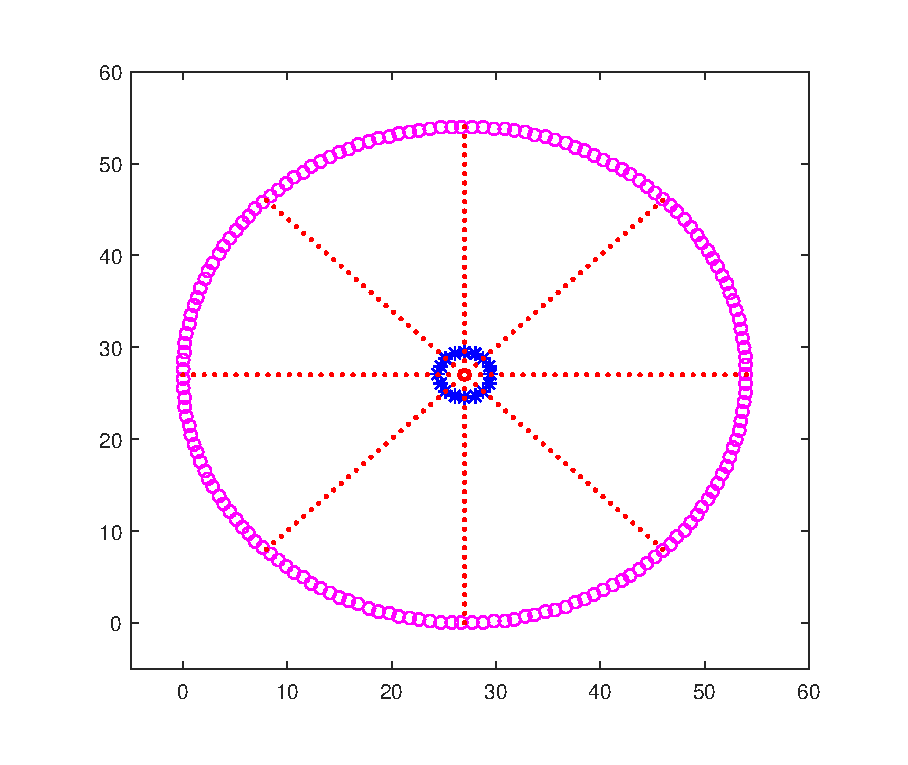
\includegraphics[height=9.0cm, width=10.0cm]{img/draw_sky_wheel.eps}
    \caption{摩天轮初始状态排布图}
    \label{摩天轮初始状态}
\end{figure}
在该布局中,将摩天轮分解为三个基本元素,并将其映射到笛卡尔坐标系中,可以得到每个基本元素满足的方程为
\begin{gather}
    \label{摩天轮材料计算公式1}
    c_1+C_1+4d=400\\
    \label{摩天轮材料计算公式2}
    d\pi=C_1
\end{gather}
其中$c_1$为小圆的周长,$C_1$为大圆的周长,$d$为线型结构的长度。易推导得到一个比例大小较为合适的结果为
\begin{table}[h]
    \vspace{20pt}
    \centering
    \caption{摩天轮所需无人机数目}
    \begin{tabular}{p{2cm}p{3cm}}
        \hline
        元素            &   尺寸(个) \\
        \hline 
        小圆            &   16*1 \\
        大圆            &   168*1 \\
        线段            &   56*8 \\
        \hline
    \end{tabular}
    \label{摩天轮所需无人机数目}
\end{table}
在无人机进行起飞之前所需场地由摩天轮这一画面所决定,可以使用很少的占地面积,也方便之后的画面切换。根据计算,当大圆直径$d$为56单位无人机时,所需占地面积为无人机直径$df=0.3m$与单位数的乘积。则起飞所需占地面积为:
\begin{align*}
    S &= (\frac{df\times d}{2})^2 \times \pi\\
    & = (\frac{0.3 \times 56}{2})^2 \times \pi\\
    & = 221.7m^2
\end{align*}
当无人机起飞后,考虑到无人机之间的相互影响,以及灯光秀时两个发光无人机灯效的连接性,可以将无人机尺寸模型估计为直径$df$为$0.5m$的圆,这样可以尽可能扩大表演空间,也可以很好的保证表演效果不至于特别散。那么在起飞过程中,根据无人机发散飞行参数可以推导得出最终的天空所占区域面积为:
\begin{align*}
    S &= (\frac{df\times d}{2})^2 \times \pi\\
    & = (\frac{0.5 \times 56}{2})^2 \times \pi\\
    & = 615.8m^2
\end{align*}
\subsubsection{功夫熊猫起飞布局}
\begin{figure}[htbp]
    \centering
    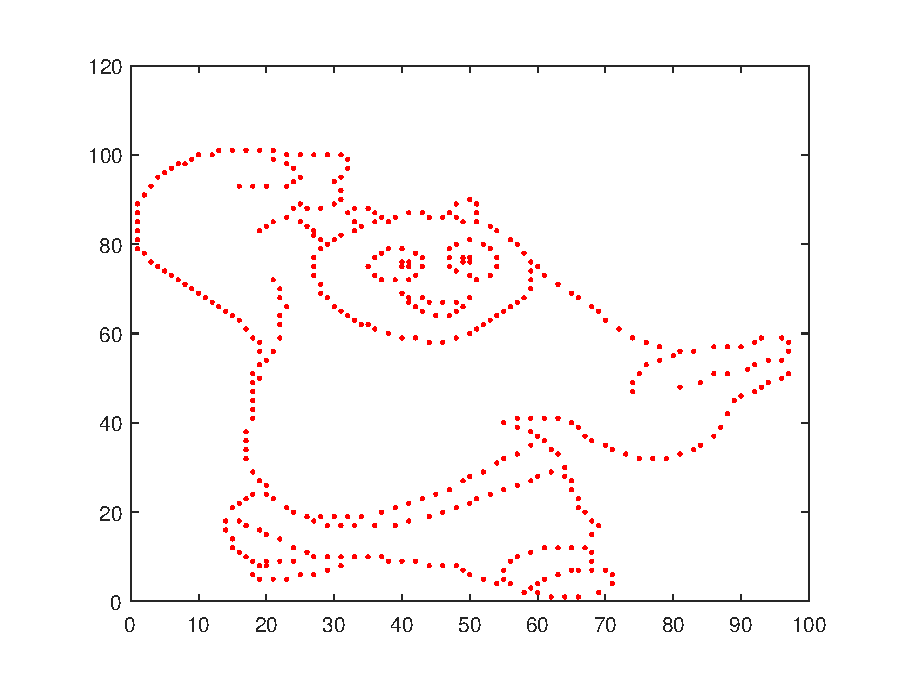
\includegraphics[height=9.0cm,width=10.0cm]{img/draw_panda.eps}
    \caption{功夫熊猫排布图}
    \label{功夫熊猫排布}
\end{figure}
功夫熊猫形状数据由题目给出,将其读出并映射到笛卡尔坐标系中可以得到如图\ref{功夫熊猫排布}所示结果。
由于该画面不在地面活动,仅在天空进行表演,在所给数据中,数据大小为$101\times97$,无人机升空后模型仍等效为直径$df$为$0.5m$的圆。所以其占地面积计算由所给数据可直接计算得出:
\begin{align*}
    S = 101 \times 0.5 \times 97 \times 0.5=99m^2
\end{align*}
\subsubsection{CUMT起飞布局}
在该布局中,仍然采用分割元素的方法将其拆分为一个一个的小元素,然后将其拼接完成形成一个完整的图,其完整的排布效果如下图\ref{CUMT排布}所示。
\begin{figure}[htbp]
    \centering
    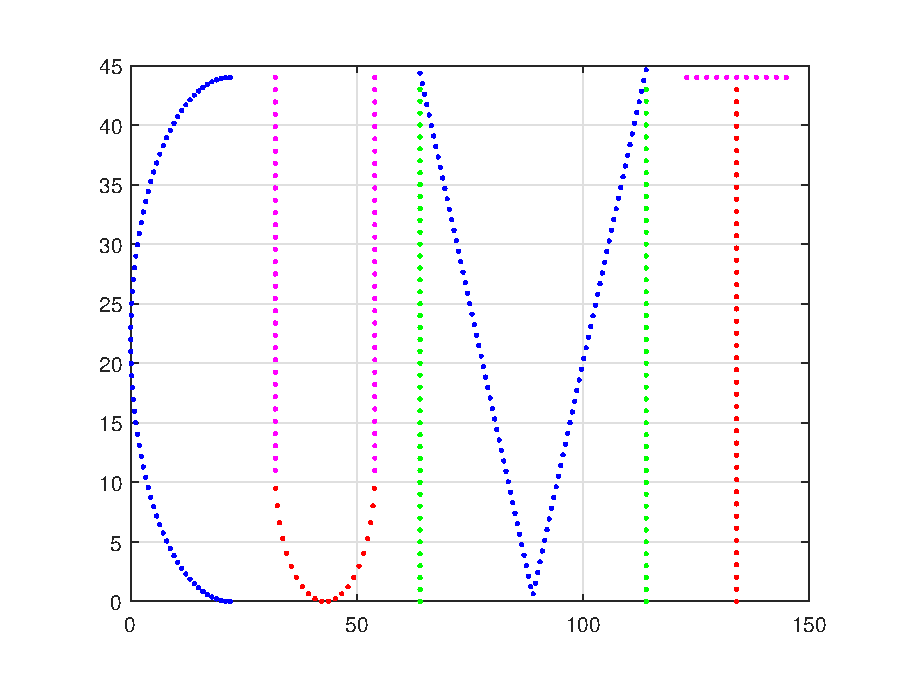
\includegraphics[height=6.0cm,width=12.0cm]{img/draw_cumt.eps}
    \caption{CUMT排布图}
    \label{CUMT排布}
\end{figure}
该图可完整拆分为两个半圆和七条直线,根据该结果计算每个元素所需的无人机数目:
\begin{equation}
    \label{CUMT计算}
    \left\{
        \begin{array}{c}
            \frac{1}{2}\pi d_1 + \frac{1}{2}\pi d_2 + 2l_2 + 2l_{3_1} + 2l_{3_2} + l_{4_1} + l_{4_2}=400 \\
            d_1=2d_2\\
            l_{3_2}=\frac{2}{\sqrt{3}}l_{3_1}\\
            l_{4_1}=\frac{1}{2}l_{4_2}
        \end{array}
        \right.
\end{equation}
根据方程组\eqref{CUMT计算}可计算得到下表\ref{CUMT布局表}参数。
\begin{table}
    \centering
    \vspace{20pt}
    \caption{CUMT布局各个参数}
    \begin{tabular}{p{2cm}p{5cm}}
        \hline
        参数    &   所需无人机单位数(个)\\
        \hline
        $d_1$   &   69\\
        $d_2$   &   35\\
        $l_2$   &   22\\
        $l_{3_1}$   &   44\\
        $l_{3_2}$   &   50\\
        $l_{4_1}$   &   22\\
        $l_{4_2}$   &   44\\
        \hline
    \end{tabular}
    \label{CUMT布局表}
\end{table}
在该布局下,每个无人机升空后仍等效为一个直径$df$为$0.5m$的圆形。在每个节点处均设置唯一一个无人机,防止有无人机的位置交叉。
\subsection{问题2:规划无人机飞行轨迹}
\subsection{粒子群算法}
粒子群算法模拟鸟群随即搜寻事物的捕食行为,用于解决优化问题。在粒子群算法中,每个优化问题的潜在解都可以想象成搜索空间的一只鸟,称之为“粒子”。所有的粒子都有一个被优化的函数决定的适应度值,每个粒子还有一个函数决定他们的飞行方向和距离。然后粒子就在当前最优解空间中搜索。
粒子群算法初始化一群随机粒子,然后通过迭代找到最优解。在每一次迭代过程中,粒子通过跟踪两个极值来更新自己:第一个就是粒子本身所找到的最优解,这个解称为个体极值,另一个极值是整个种群目前找到的最优解,这个极值是全局极值。\cite{基于GPU的大规模无人机编队控制并行仿真方法}

假设在一个$d$维的目标搜索空间中,有$n$个粒子组成一个群落,其中第$i$个粒子是一个$d$维向量:
\begin{equation}
    X_i=(x_{i1}, x_{i2}, ... x_{id}), i=1, 2, 3, ...,n
\end{equation}
第$i$个粒子的飞行速度也是一个$d$维向量,记为
\begin{equation}
    V_i=(v_{i1}, v_{i2}, v_{i3}, ..., v_{id}), i=1, 2, 3, ...,n
\end{equation}
第$i$个粒子搜索到的最优位置称为个体极值,记为
\begin{equation}
    P_{best}=(p_{i1}, p_{i2}, p_{i3},..., p_{id}), i=1, 2, 3, ...,n
\end{equation}
整个粒子群搜索到的最优位置为全局极值,记为
\begin{equation}
    g_{best}=(p_{g1}, p_{g2}, ..., p_{gd})
\end{equation}
在找到这两个最优值时,粒子根据式\ref{速度更新式子}、式\ref{位置更新位置}、来更新自己的速度和位置
\begin{gather}
    v_{id}=wv_{id}+c_1r_1(p_{id}-x_{id})+c_2r_2(p_{gd}-x_{id}) \label{速度更新式子}\\
    x_{id}=x_{id}+v_{id}\label{位置更新位置}
\end{gather}
\subsubsection{基于粒子群算法的无人机路径规划}
无人机的路径规划目的是在满足燃料消耗、安全区域的约束条件下,为无人机规划出一条从起始点到目标点评价最高的一条路径。飞行路径规划是一个空间搜索问题,主要是分为启发式算法和进化算法。其中的启发式算法由于搜索空间大,计算量大,并且规划效果对启发函数的依赖性强;进化算法是一种基于种群的优化算法,常用的算法有蚁群算法、遗传算法等。这些算法在一定程度上有很大缺陷,比如搜索量大、效率不高等问题。所以在此处使用粒子群算法进行无人机的路径规划。\cite{基于优化粒子群算法的无人机航路规划}
\section{总结}
基于粒子群算法的无人机路径规划算法可以很大程度上优化在安全区域、燃料消耗限制条件下的路径规划问题,并且可以在计算量不是很大、计算难度不是很高的情况下快速取得最优解。理论证明,基于粒子群的路径规划算法是一种相对有效和优越的解决方法。
\newpage
\bibliographystyle{unsrt} 
\bibliography{refdb} 
\newpage
\section{附录代码}
\lstset{language=matlab}
\begin{lstlisting}
    %% 无人机灯光秀数学建模无人机绘图
    % 作者:胡小忠
    % 日期:2019年4月5日
    
    %% 初始化工作空间
    clear;close all;clc;
    
    %%  绘制摩天轮原有布局
    figure(1);
    D = 54;d = 5;
    R = D / 2;r = 5 / 2;
    theta = linspace(0, 2 * pi, 168);
    x = R * cos(theta);
    y = R * sin(theta);
    plot(x + R, y + R, 'om');
    hold on;
    theta = linspace(0, 2 * pi, 17);
    x = r * cos(theta);
    y = r * sin(theta);
    plot(x + R, y + R, '*b');
    x = linspace(-19, 19, 54);
    plot(x + R, x + R, '.r');
    plot(x + R, -x + R, '.r');
    x = linspace(-27, 27, 54);
    plot(0 + R, x + R, '.r');
    plot(x + R, 0 + R, '.r');
    axis([-5, 60, -5, 60])
    %% 绘制功夫熊猫原有布局
    figure(2);
    data = xlsread('./data.xlsx');
    [height, width] = size(data);
    x = zeros(1, []);
    y = zeros(1, []);
    x_i = 1;
    y_i = 1;
    for j = 1:height
        for i = 1:width
            if data(height - j + 1, i) == 1
                x(x_i) = i;
                y(y_i) = j;
                x_i = x_i + 1;
                y_i = y_i + 1;
            end
        end
    end
    plot(x, y, '.r');
    
    %% 绘制CUMT原有布局
    figure(3);
    theta = linspace(pi/2, 3/2 * pi, 69);
    x = 22 + 22 * cos(theta);
    y = 22 + 22 * sin(theta);
    plot(x, y, '.b');
    hold on;
    grid on;
    theta = linspace(pi, 2 * pi, 24);
    x = 43 + 11 * cos(theta);
    y = 11 + 11 * sin(theta);
    plot(x, y, '.r');
    plot(32, linspace(11, 44, 33), '.m');
    plot(54, linspace(11, 44, 33), '.m');
    plot(64, linspace(0, 43, 44), '.c');
    plot(114, linspace(0, 43, 44), '.c');
    x = linspace(64, 88.5, 50);
    y = -1.76 * x + 157;
    plot(x, y, '.b');
    x = linspace(89, 114, 50);
    y = 1.76 * x + -156;
    plot(x, y, '.b');
    plot(134, linspace(0, 44, 44), '.r');
    plot(linspace(123, 145, 11), 44, '.m');
\end{lstlisting}
\end{document}